% 双曲函数
% 双曲函数|指数函数|反函数

\pentry{指数函数}

这里介绍三种双曲函数:双曲正弦函数, 双曲余弦函数和双曲正切函数, 他们的定义分别为
\begin{align}
\sinh x &= \frac{\E^x - \E^{-x}}{2}\\
\cosh x &= \frac{\E^x + \E^{-x}}{2}\\
\tanh x &= \frac{\sinh x}{\cosh x} = \frac{\E^x - \E^{-x}}{\E^x + \E^{-x}}
\end{align}
其中 $\E$ 是一个高等数学中常见的常数, 叫做自然对数底\upref{E}. 这三个函数的图像如\autoref{TrigH_fig1}.

\begin{figure}[ht]
\centering
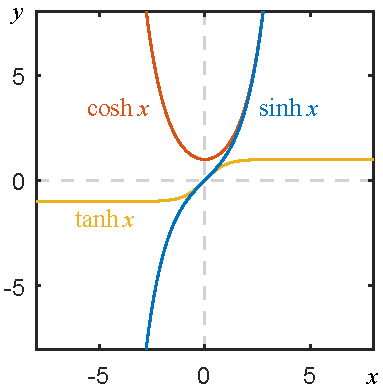
\includegraphics[width=6cm]{./figures/TrigH1.pdf}
\caption{三种双曲函数的图像} \label{TrigH_fig1}
\end{figure}

注意 $\sinh x$ 和 $\tanh x$ 是奇函数, $\cosh x$ 是偶函数.

\begin{example}{反双曲正弦函数}\label{TrigH_ex1}
要求 $\sinh x$ 的反函数, 我们令
\begin{equation}
x = \sinh y =  \frac{\E^y - \E^{-y}}{2}
\end{equation}
整理成关于 $\E^y$ 的二次方程, 得
\begin{equation}
(\E^y)^2 - 2x \E^y - 1 = 0
\end{equation}
解出 $\E^y$ 为
\begin{equation}
\E^y = x \pm \sqrt{x^2 + 1}
\end{equation}
由于 $\E^y > 0$, 上式取正号. 两边取自然对数, 得
\begin{equation}
y = \sinh^{-1} x = \ln(x + \sqrt{x^2 + 1})
\end{equation}
\end{example}
